\documentclass[11pt]{article}
\usepackage[utf8]{inputenc}
\usepackage[T1]{fontenc}
\usepackage{graphicx}
\usepackage[export]{adjustbox}
\graphicspath{ {./images/} }

\begin{document}
Overview of Financial Structuring

In the context of alternative investments, structuring is the process of engineering unique financial opportunities from existing asset exposures. An example of a structured product is an investment specially designed to provide downside protection against losses while offering potential profits through exposure to increases in the value of an index or an underlying portfolio.

Financial structuring enables different investors to hold claims with different risk exposures (or other characteristics) from the same underlying assets. This lesson provides an overview. The most common major structuring of assets is the typical capital structure of the corporate form of business organization. This capital structure partitions the risks of the corporation's underlying assets into claims of relatively low risk (e.g., debt) and relatively high risk (equity), as illustrated in the next exhibit.

The typical capital structuring of a business enterprise into debt and equity claims captures the most fundamental concepts and motivations to financial structuring: tailoring the risks of securities to the risk preferences of investors.

The capital structure of a traditional operating firm, illustrated in the next exhibit, is a very common application of the concept of structuring for risk purposes. The risk purpose served by a firm's capital structure is that the risk of the firm's assets is partitioned among the firm's capital providers. Different security classes in the firm are primarily differentiated by their levels of risk. Structuring risk is the primary motivation to the structured products discussed in the sessions from Introduction to Structuring through Equity-Linked Structured Products. Structuring may be used to differentiate ownership on attributes other than risk. Taxation can play an important role in structuring. The idea is to divvy up the claims to an asset, with cash flows being distributed based on aggregate tax minimization. In that scenario, highly taxed cash flows are distributed to tax-exempt investors or investors in low tax brackets, while tax-advantaged cash flows are distributed to investors in high tax brackets.

Structuring can also accommodate other preferences, such as those involving liquidity. Heterogeneous liquidity preferences are accommodated by structuring an asset into short-term claims for investors who place a high value on liquidity and long-term claims for investors less concerned about liquidity.

\begin{center}
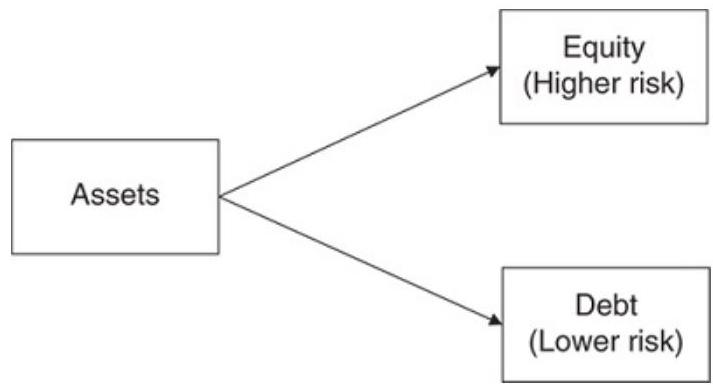
\includegraphics[max width=\textwidth]{2024_04_09_9bf8a7f77f11effcb65bg-2}
\end{center}

Capital Structure as Creating Structured Products


\end{document}